\documentclass[answers]{exam}

%% Language and font encodings
\usepackage[english]{babel}
\usepackage[utf8x]{inputenc}
\usepackage[T1]{fontenc}
% \usepackage{enumitem}
%% Sets page size and margins
\usepackage[a4paper,margin=2cm]{geometry}

%% Useful packages
\usepackage{amsmath}
\usepackage{amssymb}
\usepackage{graphicx}
\usepackage{paralist}
\usepackage{framed}
\usepackage{tikz}
\usepackage{float}
\usepackage{listings}
\usepackage{xcolor}
\tikzset{
  % define the bar graph element
  bar/.pic={
    \fill (-.1,0) rectangle (.1,#1) (0,#1) node[above,scale=1/2]{$#1$};
  }
}
\definecolor{codegreen}{rgb}{0,0.6,0}
\definecolor{codegray}{rgb}{0.5,0.5,0.5}
\definecolor{codepurple}{rgb}{0.58,0,0.82}
\definecolor{backcolour}{rgb}{0.95,0.95,0.92}
% Colored Python listing from https://www.overleaf.com/learn/latex/Code_listing
\definecolor{codegreen}{rgb}{0,0.6,0}
\definecolor{codegray}{rgb}{0.5,0.5,0.5}
\definecolor{codepurple}{rgb}{0.58,0,0.82}
\definecolor{backcolour}{rgb}{0.95,0.95,0.92}
 
\lstdefinestyle{mystyle}{
    backgroundcolor=\color{backcolour},   
    commentstyle=\color{codegreen},
    keywordstyle=\color{magenta},
    numberstyle=\tiny\color{codegray},
    stringstyle=\color{codepurple},
    basicstyle=\ttfamily\footnotesize,
    breakatwhitespace=false,         
    breaklines=true,                 
    captionpos=b,                    
    keepspaces=true,                 
    numbers=left,                    
    numbersep=5pt,                  
    showspaces=false,                
    showstringspaces=false,
    showtabs=false,                  
    tabsize=2
}
\lstset{style=mystyle}

\usetikzlibrary{matrix}

\setlength\FrameSep{4pt}

\begin{document}
    \section*{Q4. Saying Random is not enough}

%--------------------------------  4.1  ------------------------------------
    \subsection*{4.1}
    \begin{framed}
        \begin{enumerate}
            \item \emph{random\_theta()}: The function finds random $\theta_1$ and $\theta_2$. $\theta$ is chosen randomly from degrees($\phi$) and then converted to radians.\\
                    \begin{align*}
                        \theta_1 &= \phi_1 . \frac{\pi}{180}\\
                        \theta_2 &= \phi_2 . \frac{\pi}{180}
                    \end{align*}
            \item \emph{cord(R)}: The function takes the radius as the input and returns length of the cord between $\theta_1$ and $\theta_2$. It first calls \emph{random\_theta()}, and find the absolute value of their difference ($\theta=|\theta_1 - \theta_2|$). Then the length of the cord in calculated using the following formuls,\\
                    $$\text{cord length}=2R.\sin(\theta/2)$$
            \item \emph{find\_cords1(R)}: The function takes radius R as input, then draw the histogram as the output. It iterates 1000 times, calls \emph{cord(R)} for each iteration and append the result in \emph{cord\_len}. Then we calculate the value of appropriate bins for the histogram, and then plot it using matplotlib.
        \end{enumerate}
    \end{framed}
    \lstinputlisting[firstline=4,lastline=30,language=python]{Q4.py}
    \begin{figure}[h]
        \caption{Histogram of 4.1}
        \centering
        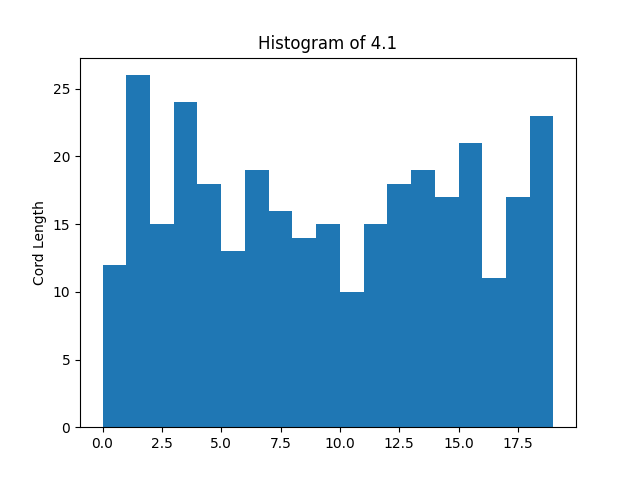
\includegraphics[scale=0.7]{Q4/Q4(1).png}
    \end{figure}

%--------------------------------  4.2  ------------------------------------
    \subsection*{4.2}
    \begin{framed}
        
    \end{framed}
    \lstinputlisting[firstline=31,lastline=65,language=python]{Q4.py}
    \begin{figure}[h]
        \caption{Histogram of 4.2}
        \centering
        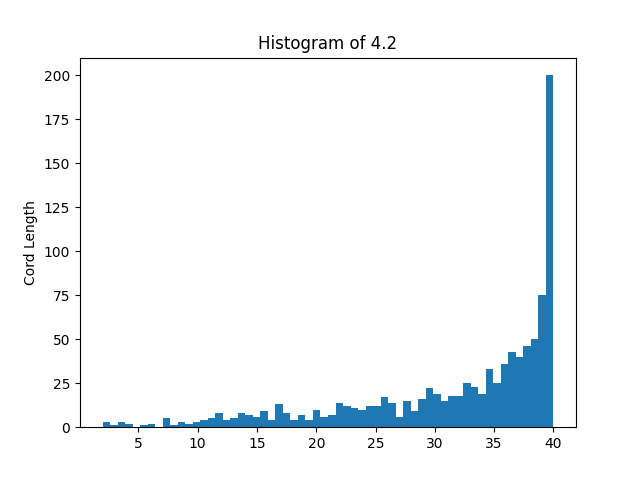
\includegraphics[scale=0.7]{Q4/Q4(2).png}
    \end{figure}
%--------------------------------  4.3  ------------------------------------
    \subsection*{4.3}
    \begin{framed}
        
    \end{framed}
    \lstinputlisting[firstline=66,lastline=106,language=python]{Q4.py}
    \begin{figure}[h]
        \caption{Histogram of 4.3}
        \centering
        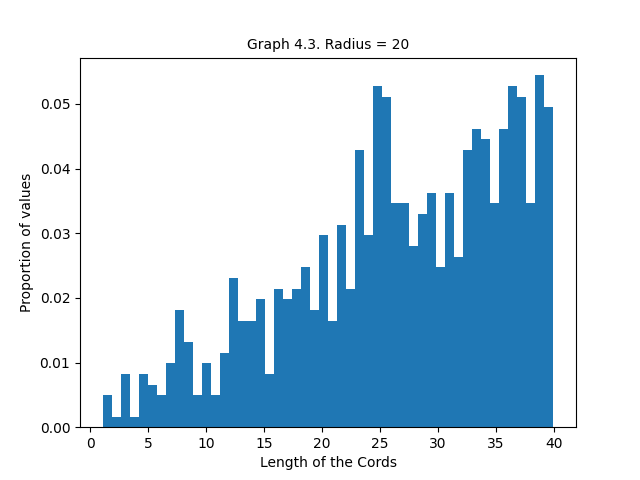
\includegraphics[scale=0.7]{Q4/Q4(3).png}
    \end{figure}
\end{document}